\documentclass{article}
\usepackage{amsmath,amstext,amssymb}
\usepackage[ttscale=0.7]{libertine}
\usepackage[libertine]{newtxmath}
\usepackage{siunitx}
\usepackage{inconsolata}
\usepackage{wrapfig}

\usepackage{sectsty}
\allsectionsfont{\sffamily}

\usepackage{xcolor}
\usepackage[colorlinks=true,
            linkcolor=blue,
            urlcolor=blue,
            breaklinks,
            pdftex,
            allbordercolors=white]{hyperref}
\usepackage{graphicx}
\usepackage{booktabs}
\usepackage{chemformula}
\usepackage{parskip}

\usepackage{listings}

\usepackage{datetime2}
\renewcommand{\DTMdisplaydate}[4]{#1-#2-#3}

\begin{document}

\lstset{language=XML,stringstyle=\ttfamily}

\begin{center}
	\Large{\textbf{\sffamily{THAMES v5.0 Output Guide}}}
\end{center}
\begin{center}
	\large{Jeffrey W. Bullard}
\end{center}
\begin{center}
	\large{\DTMnow}
\end{center}

\vspace{0.25truein}
\tableofcontents

\vspace{0.25truein}
This document provides guidance on the information contained in the various output files
produced by THAMES v5.0. For simplicity, the guide will be structured entirely
in the form of an example simulation based on the test case named
\verb!portcem-296K-sealed-alk-wc45! that is provided.

\section{\label{sec:assumption} Assumptions}
This guide assumes
\begin{enumerate}
	\item that you have the THAMES 5.0 distribution located in a directory
	      with the absolute path specified in this guide by \verb!$THAMES!. For example
	      if your distribution is located at the absolute path
	      \verb!/home/odehwah/models/THAMES!, then \verb!$THAMES! is equivalent to that
	      full path in this guide; and
	\item that you have already built \verb!thames! and that it is in
	      your \verb!$PATH! environment variable so that the operating system can discover it
	      when you run it from the command line. If you are unsure whether this has been
	      done, you can run the command \verb!which thames! from the command line. If that
	      command returns something like \verb!thames not found!, then you must first
	      augment your \verb!$PATH! environment variable. If you are unsure how to
	      change the environment variable a tutorial for Linux can be found
	      here: \url{https://www.digitalocean.com/community/tutorials/how-to-view-and-update-the-linux-path-environment-variable}
\end{enumerate}

\section{\label{sec:categories} Run the Test Case}
A good idea is to keep the working directory as clean as possible so that it
doesn't get accidentally corrupted or more confusing. So it is a good practice
to copy the test case to another location before using it there. For this
example, create a temporary directory and then copy the test case there:
\scriptsize{
	\begin{lstlisting}
  mkdir $HOME/scratch
  cp -R $THAMES/test/portcem-296K-sealed-alk-wc45 $HOME/scratch
\end{lstlisting}
}

\normalsize{ }
Next, go to that new directory:
\scriptsize{
	\begin{lstlisting}
  cd $HOME/scratch/portcem-296K-sealed-alk-wc45
\end{lstlisting}
}

\normalsize{ }
Before running the simulation, open the \verb!input.in! file. The file contents
are:
\scriptsize{
	\begin{lstlisting}
2
thames-dat.lst
simparams.json
ccr140-w45-thames.img
cem140-sealed-alk-01
\end{lstlisting}
}

\normalsize{ }
Each line of this file is now explained:
\begin{itemize}
	\item \textbf{Line 1}: Determines the type of simulation to be run:
	      \begin{enumerate}
		      \item A value of 1 exits the simulation with no further action
		      \item A value of 2 will run a normal hydration simulation
	      \end{enumerate}
	\item \textbf{Line 2}: The root name of the thermodynamic data. This file is
	      read and automatically prompts the input of the other thermodynamic data
	      files.
	\item \textbf{Line 3}: The JSON formatted input file specifying the simulation
	      environment, the microstructure phase definitions, and the simulation time
	      and output frequency.
	\item \textbf{Line 4}: The name of the file containing the initial 3D microstructure
	\item \textbf{Line 5}: The root name for all output files produced by THAMES.
	      This can be anything you want, although it is recommended not to use periods
	      within it. Feel free to shorten it to \verb!cem140! or some other string if
	      you wish.
\end{itemize}
Close the file, making sure to save it first if you made changes to the fifth
line, and then run the THAMES simulation with these options:
\scriptsize{
	\begin{lstlisting}
  thames --xyz --outfolder MyResult < input.in >& output.out &
\end{lstlisting}
}

\normalsize{ }
The simulation should create an \verb!output.txt! file and a folder named
\verb!MyResults!, as shown in Figure~\ref{fig:one}, while it continues
to run for about five minutes to ten minutes.

\begin{figure}
	\centering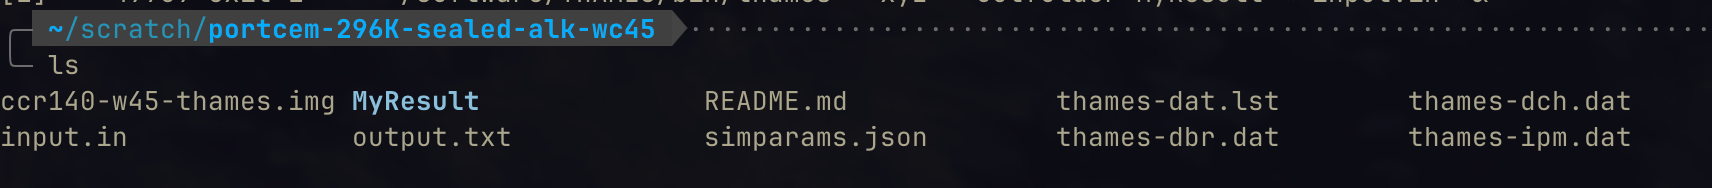
\includegraphics[width=0.7\textwidth]{../Figures/ListingAfterRun.png}
	\caption{\label{fig:one} Contents of the test directory running a simulation.}
\end{figure}

A message similar to the following
appear in the terminal when the simulation finishes:
\scriptsize{
	\begin{lstlisting}
  [1]  + 56549 exit 1     ~/Software/THAMES/bin/thames --xyz --outfolder MyResult < input.in >&
\end{lstlisting}
}

\normalsize{ }
The \verb!MyResults! folder
holds all of the output files created by the simulation, while the
\verb!output.txt! file holds all the standard output that would otherwise
be written to the screen. Under ordinary circumstances there is no need to
examine the \verb!output.txt! file, but it can be useful to have it if
the program crashes for some reason or otherwise behaves oddly.

\section{\label{sec:outputfiles} Output File Content}
When the simulation exits, navigate to the \verb!MyResults! folder and
run the \verb!ls! command to see the directory contents, which should
appear like that shown in Fig.~\ref{fig:two}.

\begin{figure}
	\centering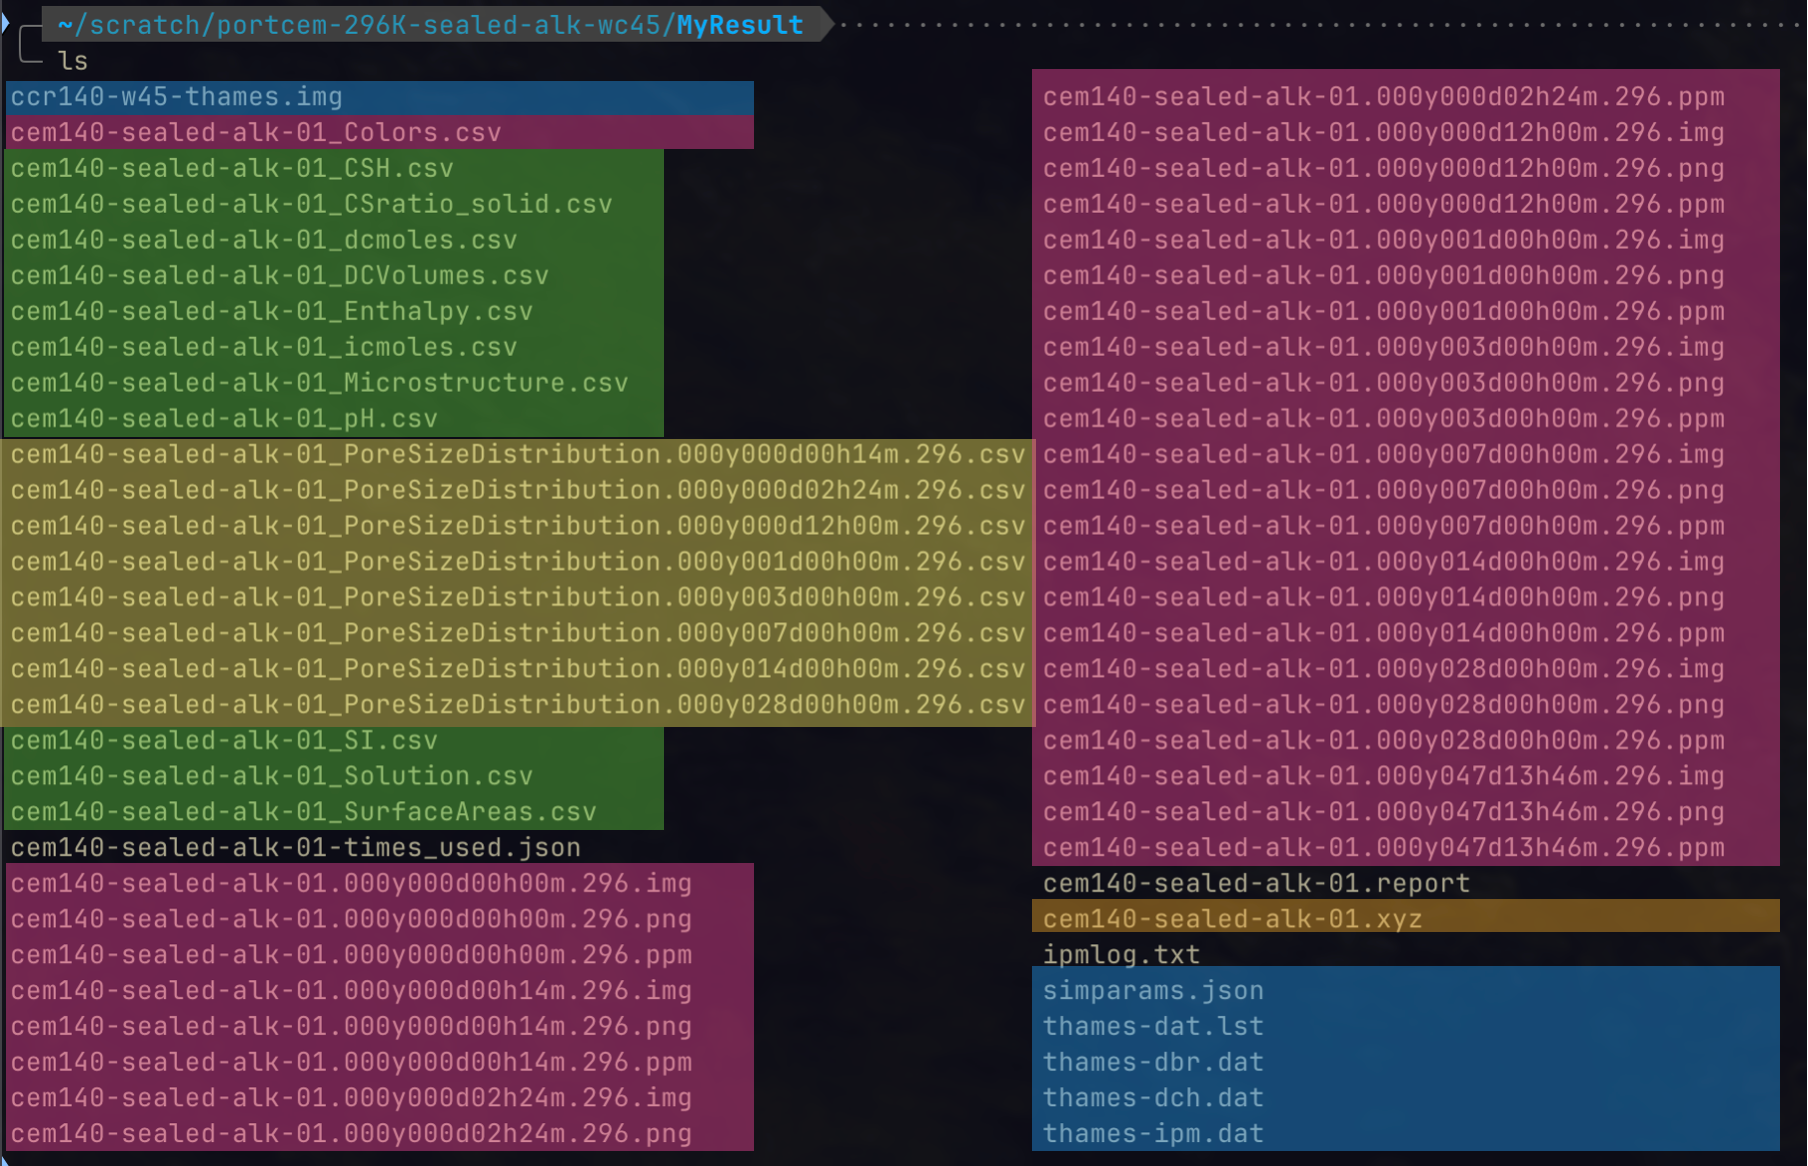
\includegraphics[width=0.7\textwidth]{../Figures/OutputFileTypes.png}
	\caption{\label{fig:two} Contents of the \texttt{MyResult} folder at the
		conclusion of THAMES simulation. Color blocks superimposed on the files
		indicate spreadsheet-like CSV data (green), pore size distribution data
		(yellow), microstructure data and images for viewing (pink), a 3D
		\texttt{xyz}
		format file for viewing in Ovito or similar application (orange, optional),
		and original input data files (blue) copied from the parent directory for
		record-keeping.}
\end{figure}

\subsection{Input data files}
The files highlighted in blue in Fig.~\ref{fig:two} are input files
copied directly from the parent directory and are present only as
metadata to recall the conditions under which the simulation was
performed. The contents of most of these files are described in detail
in the companion document on preparing input files and will therefore
not be revisited here.

\subsection{CSV files}
Eleven comma separated value CSV files are written by THAMES to
recored time-dependent simulation data. These are highlighted in green in
Fig.~\ref{fig:two} and are described in the following paragraphs:

\paragraph{\_CSH.csv} Records the composition of the calcium silicate
hydrate (\ch{C-S-H}) phase as a function of time. The first column is the time (in hours).
The rest of the columns up until the final column are the concentrations
of each element in the \ch{C-S-H} phase. The final column displays the
molar Ca/Si ratio of the \ch{C-S-H}.

\paragraph{\_CSratio\_solid.csv} Provides the overall molar Ca/Si ratio of all
solid components in the microstructure. Time (in hours) is in the first column
and the only other column is the averaged Ca/Si ratio. This file may be
removed in future versions of THAMES.

\paragraph{\_dcmoles.csv} Catalogs the number of moles (per \qty{100}{\gram}
of initial solid) of each dependent component (DC)\footnote{Note that DCs are
	not identical with phases. Some phases, such as gypsum, have only one
	DC, which for gypsum is named \texttt{Gp}, while phases such as \ch{C-S-H}
	are solid solutions of multiple DCs.}
in the system, again with
simulation time (in hours) occupying the first column.

\paragraph{\_DCVolumes.csv} Provides the volume (in \unit{\meter\cubed} per
\qty{100}{\gram} of initial solid) of each dependent component (DC) in the
system, again with simulation time (in hours) occupying the first column.

\paragraph{\_Enthalpy.csv} Displays in the second column the predicted cumulative heat release
by the system (in \unit{\joule} per \qty{100}{\gram} of initial solid) at each
corresponding time (in hours) in the first column.

\paragraph{\_icmoles.csv} Gives the calculated moles, per \qty{100}{\gram}
of initial solid, of each independent
component (IC, essentially chemical elements and electric charge) in the system
for each corresponding time (in hours) in the first column. This file may be
removed in future versions of THAMES because it duplicates information that
can be easily obtained from the \verb!_dcmoles.csv! file.

\paragraph{\_Microstructure.csv} Records the \textit{volume fraction}
(dimensionless) of each defined microstructure phase in the system
at the corresponding time (in hours) displayed in the first column.
The very last column gives the predicted chemical shrinkage value at the
corresponding time, in units of \unit{\meter\cubed} per \qty{100}{\gram}
of initial solid material.

\paragraph{\_SI.csv} Contains the saturation index of the pore solution
(dimensionless) with respect to each defined microstructure phase
at each corresponding time (in hours) in the first column. Here the saturation
index, $\Omega$, is defined as the ratio of the activity product to the equilibrium
constant, so for any given solid phase $p$, $\Omega_p = 1$ if the solution is at
equilibrium with that solid phase, $\Omega_p < 1$ if the solution is
undersaturated so that the phase $p$ is thermodynamically driven to dissolve,
and $\Omega_p >$ if the solution is
supersaturated so that the phase $p$ is thermodynamically driven to precipitate.

\paragraph{\_Solution.csv} Displays the composition of the electyrolyte
(\textit{i.e.}, pore solution) at each calculated time (in hours) given in
the first column. The composition consists of the concentration of each
dependent component dissolved in the water, given in units of
\unit{\mole\per\kilo\gram} water.

\paragraph{\_SurfaceAreas.csv} Displays the solid-water surface
area of each defined microstructure phase at each calculation time (in hours)
displayed in the first column. The surface areas in this file are given
in units of \unit{\meter\squared} per \qty{100}{\gram} of initial solid
material. In particular, they are not equivalent to the specific surface
area of each phase individually, but come closer to reflecting each phase's
contribution to the specific surface area.

\subsection{Pores size distribution data files}
One of these files is created for each output time the user specifies in the
input JSON file, which is described in more detail in the companion guide
for preparing input files. Each file has a name that contains the
simulation temperature in kelving units and the time in year-day-hour-minute format.
For example, a file with the name
\scriptsize{
	\begin{lstlisting}
myfile_PoreSizeDistribution.001y.056d.14h.30m.296K.csv
\end{lstlisting}
}
\normalsize{ }
corresponds to a temperature of \qty{296}{\kelvin} and
a simulation time of 1 year, 56 days, 14 hours, and 30 minutes.
Times are always rounded to the nearest minute.

The contents of a pore size distribution file are structured
as shown below:
\scriptsize{
	\begin{lstlisting}
Time = 672 h
Capillary pore volume fraction (> 100 nm) = 0.124931
Capillary void volume fraction = 0.106074
Saturated capillary pore volume fraction = 0.0188566
Nanopore volume fraction (<= 100 nm) = 0.225517
Total pore volume fraction = 0.350448
Total void volume fraction = 0.106074
Pore size saturation data:
Diameter (nm),Volume Fraction,Fraction Saturated
1,0.0230988,1
2,0.032824,1
3,0.0241935,1
4,0.0172738,1
5,0.012644,1
.
.
.
96,0.00405697,1
99,0.00427539,1
>99,0.124926,0.893926
\end{lstlisting}
}

\normalsize{ }
The first seven lines provide overall data on the volume fraction of different
ranges of saturated pores and empty pores. Following this is the more detailed
analysis of pore volume fractions. The first column is the effective
pore diameter in  \unit{\nano\meter} units, the second column is the
volume fraction (dimensionless) of the microstructure occupied by pores of that size,
and the third column is the fraction of that pore volume occupied by the
pore solution. The data are provided up to a maximum pore diameter of
\qty{99}{\nano\meter}, and all larger pores are lumped into a final category
on the final row.

\subsection{Microstructure state files}
For each specified output time in the JSON input file, two or three files
will be created:
\begin{itemize}
	\item \verb!.img! files contain the full 3D microstructure image data
	      in exactly the same format as the input microstructure image, which
	      is discussed in detail in the companion guide for preparing input
	      files.
	\item \verb!.ppm! is a 2D $xy$-slice through the microstructure at the
	      midpoint of the $z$ dimension. The format is a color portable pixel
	      map (PPM) that can be displayed by a range of image rendering applications
	      such as Gimp (any platform, most flexible), \verb!eog! or \verb!feh! (linux),
	      Preview (Mac OS), Honeyview or i\_view (Windows).
	\item \verb!.png! is a PNG version of the corresponding \verb!.ppm! file
	      that THAMES will generate automatically only if ImageMagick 7 or later
	      \url{https://imagemagick.org/} is
	      installed on the computer and if the \verb!magick! command is in the
	      path.
\end{itemize}

The \verb!.ppm! and \verb!.png! files are created with some sense of
depth by making the pore space slightly transparent. These two files
also render each microstructure phase with a unique color. The
\verb!rgb! triplet of values for the color of each phase is given
in the \verb!_Colors.csv! file for easier reference.

\subsection{3D rendering file}
This file tends to be quite large and so it is only created if the user gives
the \verb!--xyz! option on the command line when starting a THAMES simulation.
It contains a full 3D data structure for each output time specified in the JSON
input file, and so can be rendered into individual states or produced into
an animation of the microstructure's time evolution. The file is written
in the industry-standard \verb!.xyz! format that can be read by multiple
3D rendering software applications. Among these,
Ovito (\url{https://ovito.org})\footnote{Mention of commercial products is
	for information only, and does not imply recommendation or endorsement by Texas A\&M University.}
is a freely available application that runs on any platform and is relatively easy to use.
\end{document}
